%%%%%%%%%%%%%%%%%%%%%%%%%%%%%%%%%%%%%%%%%%%
%Packages
%%%%%%%%%%%%%%%%%%%%%%%%%%%%%%%%%%%%%%%%%%%
%Content
%%%%%%%%%%%%%%%%%%%%%%%%%%%%%%%%%%%%%%%%%%%

\begin{landscape}
    \subsection{Grundglieder}
    \begingroup
    \scriptsize
    \newcommand{\ImageWidth}{70pt}
    \begin{tabularx}{\linewidth}{|p{100pt}|p{160pt}|p{60pt}|p{80pt}|p{120pt}|p{80pt}|}
          \hline
          \textbf{Benennung}
           &
          \textbf{Funktion}
           &
          \textbf{UTF\textsuperscript{1}}
           &
          \textbf{Symbol}
           &
          \textbf{Sprungantwort}
           &
          \textbf{Plot}
          \\
          \hline
          \hline
          %%%%%%%%%%%%%%%%%%%%%%%%%%%%%%%%%%%%%%%%%%%%%%%%%%%%%%%%%%%%%%%%%%%%%%%%%%%%%%%%%%%%%%%%%%%%%
          \textbf{P-Glied\textsuperscript{2}}
          \newline Proportionalglied
           &
          $y = K \cdot u$
           &
          $K$
           &
          \raisebox{-.5\height}{\includegraphics[width = \ImageWidth]{img/DIN-Symbole/Proportionalglied.png}}
           &
          $K$
           &
          \raisebox{-.5\height}{
                \resizebox{\ImageWidth}{!}{%
                      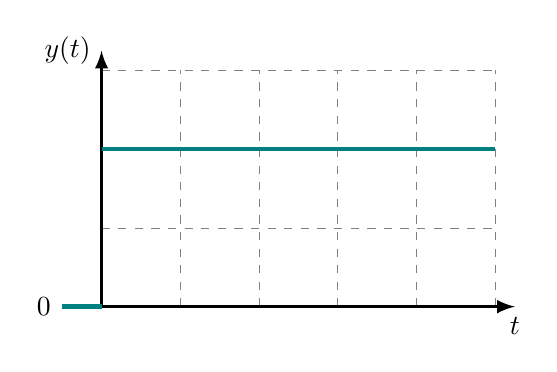
\begin{tikzpicture}
                            % Grid
                            \draw[help lines,dashed] (0,0) grid (5,3);

                            % Axes
                            \draw[very thick,latex-latex] (0,3.25) node[left]{$y(t)$}
                            |- (5.25,0) node[below]{$t$};

                            % Plot function
                            \draw[ultra thick,teal] (-0.5,0) node[left,black](s0){$0$}
                            -- ++(0.5,0)
                            plot[domain=0:5,
                                        samples = 50,
                                        smooth]({\x}, {2});
                      \end{tikzpicture}
                }
          }
          \\
          \hline
          \rowcolor{TabularBackgroundColor}
          %%%%%%%%%%%%%%%%%%%%%%%%%%%%%%%%%%%%%%%%%%%%%%%%%%%%%%%%%%%%%%%%%%%%%%%%%%%%%%%%%%%%%%%%%%%%%
          \textbf{I-Glied}
          \newline(Idealer Integrierer)
           &
          $y(t) = K \cdot \int \limits _{t=0} ^{t} u(\tau) d\tau + y(0)$
          \newline $\dot{y}(t) = K \cdot u(t)$
           &
          $K \frac{1}{s}$
           &
          \raisebox{-.5\height}{\includegraphics[width = \ImageWidth]{img/DIN-Symbole/Integrator.png}}

           &
          $K \cdot t$
           &
          \raisebox{-.5\height}{
                \resizebox{\ImageWidth}{!}{%
                      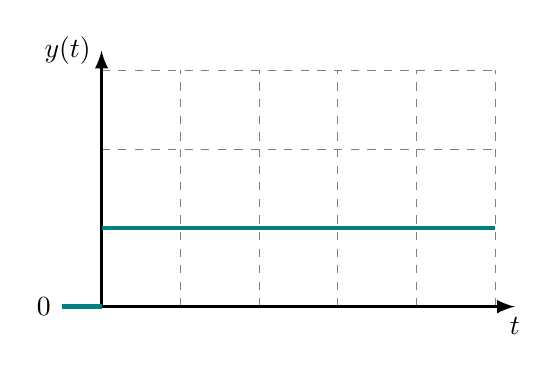
\begin{tikzpicture}
                            % Grid
                            \draw[help lines,dashed] (0,0) grid (5,3);

                            % Axes
                            \draw[very thick,latex-latex] (0,3.25) node[left]{$y(t)$}
                            |- (5.25,0) node[below]{$t$};

                            % Plot function
                            \draw[ultra thick,teal] (-0.5,0) node[left,black](s0){$0$}
                            -- ++(0.5,0)
                            plot[domain=0:5,
                                        samples = 50,
                                        smooth]({\x},);
                      \end{tikzpicture}
                }
          }
          \\
          \hline
          %%%%%%%%%%%%%%%%%%%%%%%%%%%%%%%%%%%%%%%%%%%%%%%%%%%%%%%%%%%%%%%%%%%%%%%%%%%%%%%%%%%%%%%%%%%%%
          \textbf{Totzeit-Glied}
           &
          $y(t) = u(t-T_t)$
           &
          $e^{-s T_t}$
           &
          \raisebox{-.5\height}{\includegraphics[width = \ImageWidth]{img/DIN-Symbole/Totzeitglied.png}}
           &
          $\sigma(t-T) = \begin{cases}
                                     0, t<T     \\
                                     1, t\geq T \\
                               \end{cases}$
           &
          \raisebox{-.5\height}{
                \resizebox{\ImageWidth}{!}{%
                      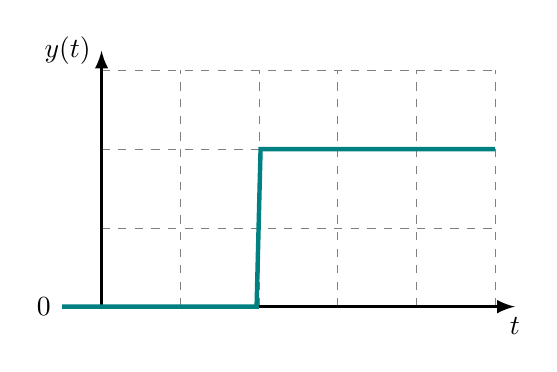
\begin{tikzpicture}
                            % Grid
                            \draw[help lines,dashed] (0,0) grid (5,3);

                            % Axes
                            \draw[very thick,latex-latex] (0,3.25) node[left]{$y(t)$}
                            |- (5.25,0) node[below]{$t$};

                            % Plot function
                            \draw[ultra thick,teal] (-0.5,0) node[left,black](s0){$0$}
                            -- ++(0.5,0)
                            plot[domain=0:5,
                                        samples = 100,
                                  ]({\x},{ (\x<=2) * 0  + (\x>2) * 2});
                      \end{tikzpicture}
                }
          }
          \\
          \hline
          \rowcolor{TabularBackgroundColor}
%%%%%%%%%%%%%%%%%%%%%%%%%%%%%%%%%%%%%%%%%%%%%%%%%%%%%%%%%%%%%%%%%%%%%%%%%%%%%%%%%%%%%%%%%%%%%
          \textbf{D-Glied}
          \newline Idealer Differenzierer
           &
          $y(t) = K \cdot \frac{du(t)}{dt} = K\cdot \dot{u}(t)$
           &
          $K \cdot S $
           &
          \raisebox{-.5\height}{\includegraphics[width = \ImageWidth]{img/DIN-Symbole/D-Glied.png}}
           &
          $K\cdot \delta(t)$
           &
          \raisebox{-.5\height}{
                \resizebox{\ImageWidth}{!}{%
                      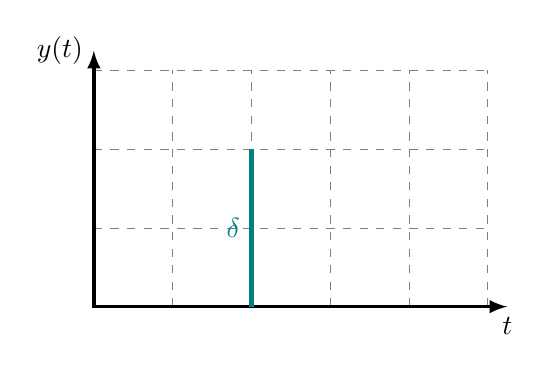
\begin{tikzpicture}
                            % Grid
                            \draw[help lines,dashed] (0,0) grid (5,3);

                            % Axes
                            \draw[very thick,latex-latex] (0,3.25) node[left]{$y(t)$}
                            |- (5.25,0) node[below]{$t$};

                            % Plot function
                            \draw[ultra thick ,teal] (2,0) -- node[left]{$\delta$} (2,2);
                            
                      \end{tikzpicture}
                }
          }
          \\
          \hline
          %%%%%%%%%%%%%%%%%%%%%%%%%%%%%%%%%%%%%%%%%%%%%%%%%%%%%%%%%%%%%%%%%%%%%%%%%%%%%%%%%%%%%%%%%%%%%
          \textbf{DT\textsubscript{1}-Glied}
          {
                \tiny 
                \newline Realisierbarer Differenzierer
                \newline K: Verstärkung
                \newline T: Zeitkonstante
          }
           &
          $ y(t) + T \cdot \dot{y}(t) = K \dot{u}(t)$
          \newline $y(t) = K \dot{u}(t) - T \cdot \dot{y}(t)$
          
           &
          $\frac{K \cdot s}{1+T_s}$
           &
          \raisebox{-.5\height}{\includegraphics[width = \ImageWidth]{img/DIN-Symbole/DT-Glied.png}}
           &
          $\frac{K}{T}\cdot e^{-\frac{t}{T}}$
           &
          \raisebox{-.5\height}{
                \resizebox{\ImageWidth}{!}{%
                      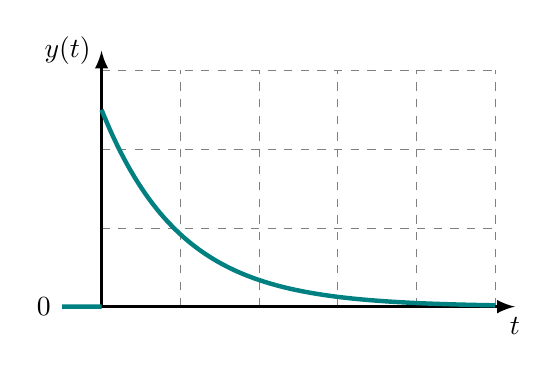
\begin{tikzpicture}
                            % Grid
                            \draw[help lines,dashed] (0,0) grid (5,3);

                            % Axes
                            \draw[very thick,latex-latex] (0,3.25) node[left]{$y(t)$}
                            |- (5.25,0) node[below]{$t$};

                            % Plot function
                            \draw[ultra thick,teal] (-0.5,0) node[left,black](s0){$0$}
                            -- ++(0.5,0)
                            plot[domain=0:5,
                                        samples = 50,
                                        smooth]({\x},{2.5*exp(-(\x))});
                      \end{tikzpicture}
                }
          }
          \\
          \hline   
          \rowcolor{TabularBackgroundColor}
          %%%%%%%%%%%%%%%%%%%%%%%%%%%%%%%%%%%%%%%%%%%%%%%%%%%%%%%%%%%%%%%%%%%%%%%%%%%%%%%%%%%%%%%%%%%%%
          \textbf{PT\textsubscript{1}-Glied}
          {
                \tiny \newline K: Verstärkung
                \newline T: Zeitkonstante
          }
           &
          $ T\dot{y} + y = K u(t)$
          \newline $T= \frac{1}{K_I \cdot K_P} $
          \newline $K = \frac{1}{K_P}$
           &
          $\frac{K}{1+T_s}$
           &
          \raisebox{-.5\height}{\includegraphics[width = \ImageWidth]{img/DIN-Symbole/PT1-Glied.png}}
           &
          $K (1-e^{-\frac{t}{T}})$
           &
          \raisebox{-.5\height}{
                \resizebox{\ImageWidth}{!}{%
                      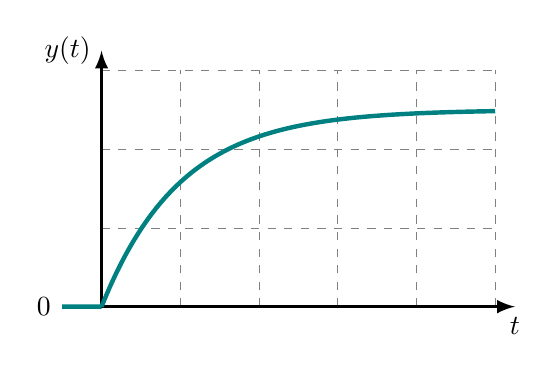
\begin{tikzpicture}
                            % Grid
                            \draw[help lines,dashed] (0,0) grid (5,3);

                            % Axes
                            \draw[very thick,latex-latex] (0,3.25) node[left]{$y(t)$}
                            |- (5.25,0) node[below]{$t$};

                            % Plot function
                            \draw[ultra thick,teal] (-0.5,0) node[left,black](s0){$0$}
                            -- ++(0.5,0)
                            plot[domain=0:5,
                                        samples = 50,
                                        smooth]({\x},{2.5*(1- exp(-(\x)))});
                      \end{tikzpicture}
                }
          }
          \\
          \hline
          %%%%%%%%%%%%%%%%%%%%%%%%%%%%%%%%%%%%%%%%%%%%%%%%%%%%%%%%%%%%%%%%%%%%%%%%%%%%%%%%%%%%%%%%%%%%%
          \textbf{PT\textsubscript{2}-Glied}
          {\tiny
                \newline K: Verstärkung
                \newline T: Zeitkonstante
                \newline $\zeta$: Dämpfungskonstante
          }
           &
          $T^2 \cdot \ddot{y}(t) + 2 \zeta T \cdot \dot{y}(t) + y(t) = K \cdot u(t)$
          \newline $y(t) = K \cdot x(t) + T^2 \cdot (-\ddot{y}(t)) - 2 \zeta T \cdot \dot{y}(t)$
          {\tiny
                      \newline $\zeta = \frac{h}{\sqrt{h^2 + \pi^2}}$
                      \newline $h = \log(\frac{y_m}{y_{\infty}})$
                }
           &
          $\frac{K}{T^2 + s^2 + 2 \zeta T s + 1}$
           &
          \raisebox{-.5\height}{\includegraphics[width = \ImageWidth]{img/DIN-Symbole/PT2-Glied.png}}
           &
          $KA(1+e^{\sigma t}(-cos(\omega t) + \frac{\sigma}{\omega}sin(\omega t)))$
          {\tiny
                      \newline $\omega = \frac{2\pi}{T_m}$
                      \newline $K = \frac{y_{\infty}}{A} $
                      \newline $\sigma = \frac{h\omega}{\pi}$
                }
           &
          \raisebox{-.5\height}{
                \resizebox{\ImageWidth}{!}{%
                      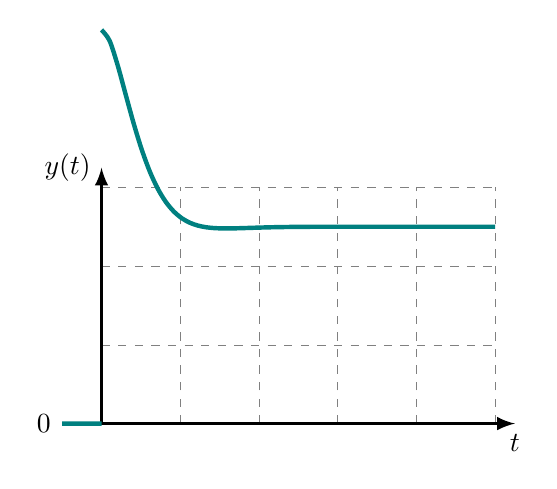
\begin{tikzpicture}
                            % Grid
                            \draw[help lines,dashed] (0,0) grid (5,3);

                            % Axes
                            \draw[very thick,latex-latex] (0,3.25) node[left]{$y(t)$}
                            |- (5.25,0) node[below]{$t$};

                            % Plot function
                            \draw[ultra thick,teal] (-0.5,0) node[left,black](s0){$0$}
                            -- ++(0.5,0)
                            plot[domain=0:5,
                                        samples = 50,
                                        %TODO: Fix this!
                                        smooth]({\x},{2.5  *   (1- exp(-3*(\x))  *  (- cos(deg(1.9848*\x)) + (-3/1.9848)*sin(deg(1.9848*\x)))  });
                            %KA = 2.5, Sigma = -3, Omega = 1.9848
                      \end{tikzpicture}
                }
          }
          \\
          \hline       
    \end{tabularx}
    \tiny{
          \\
          1. UTF = Übertragungsfunktion (Laplacetransformierte Sprungantwort)\\
          2. Proportionalglied ist einziges Statisches glied.\\
    }
    \endgroup
    \normalsize
\end{landscape}